% =========================
% Seções/1-Introdução.tex
% (não usar \section{Introdução} aqui;
%  o capítulo é aberto no main.tex)
% =========================

A resolução de problemas por \emph{busca} ocupa posição central na Inteligência Artificial (IA) simbólica: modela a 
navegação em um \emph{espaço de estados} por meio de operadores, avaliando custos e selecionando expansões 
segundo políticas informadas ou não informadas, como discutem \citeonline{russell2010artificial} e 
\citeonline{nilsson1998}. O interesse central está em compreender como diferentes algoritmos percorrem esse espaço, 
quais estruturas de dados utilizam e de que modo heurísticas afetam o desempenho.

Para fins experimentais, optou-se pelo \emph{8-puzzle} apenas como domínio de teste. Trata-se de um tabuleiro 
$3\times 3$ com oito peças móveis e um espaço vazio, no qual o objetivo é atingir uma configuração final a partir 
de um arranjo inicial (Figura~\ref{fig:8puzzle}).
\vspace{-0.2cm}
\begin{figure}[H]
    \centering
    \caption{Exemplo de níveis de busca e estados para o problema do 8-puzzle, com estado inicial, transições e estado objetivo}
    \vspace{-0.5cm}
    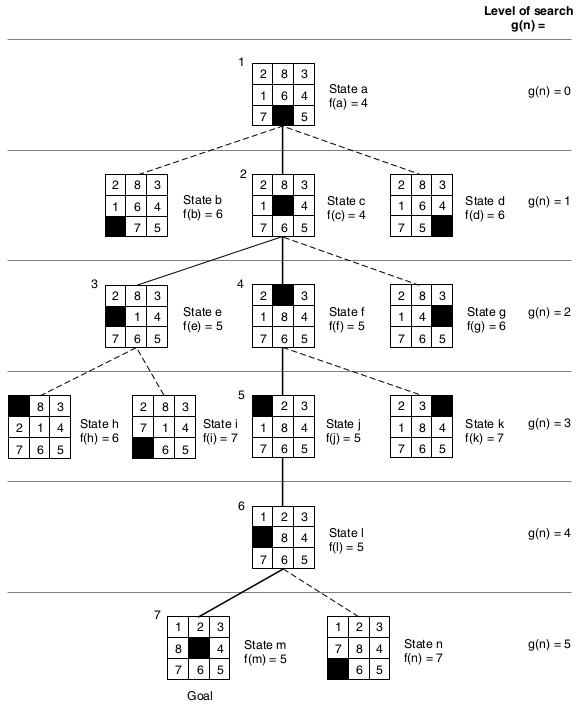
\includegraphics[width=0.56\textwidth]{Imagens/FiguraBuscaEstadosLuger.png}
    \caption*{Fonte: Extr. de \citeonline{luger2009artificial}.}
    \label{fig:8puzzle}
\end{figure}


A escolha desse problema não se deve à sua complexidade prática, mas sim ao fato de ser computacionalmente leve, permitindo implementar e comparar variações de algoritmos de busca de forma controlada e reprodutível. Assim, o foco da análise permanece nos métodos de busca --- custo uniforme e versões do algoritmo $A^*$ com heurísticas de diferentes níveis de admissibilidade --- e não no quebra-cabeça em si. Nesse sentido, o 8-puzzle funciona como um \emph{laboratório didático} que viabiliza a avaliação sistemática de desempenho.

No contexto da disciplina INE5633---\emph{Sistemas Inteligentes} (UFSC), esta Atividade Prática 1 (AP1) utiliza o 8-puzzle como laboratório para implementar e analisar o algoritmo A* e variações, em alinhamento ao conteúdo de \emph{raciocínio e resolução de problemas} e à ênfase em técnicas de procura e informação heurística; a proposta didática privilegia implementação e análise prática, em consonância com a bibliografia básica adotada \cite{russell2010artificial,luger2009artificial}.

\section{Escopo desta Atividade Prática}

Serão estudadas quatro variantes: (i) busca de custo uniforme (sem heurística), (ii) A* com heurística \emph{não admissível}, (iii) A* com heurística admissível simples e (iv) A* com a heurística admissível mais precisa desenvolvida pela equipe. A comparação considerará: total de nós visitados, comprimento do caminho-solução, maior tamanho da fronteira (abertos), tempo de execução e um arquivo \texttt{.txt}/\texttt{.json} com fronteira e visitados ao término. Esses indicadores permitem discutir \emph{admissibilidade} e \emph{consistência} das heurísticas no A*, além de seus efeitos de eficiência \cite{russell2010artificial,luger2009artificial}.

\section{Objetivos formativos}
Consolidar, por meio de implementação e experimentação reprodutível, a ponte entre teoria e prática em busca. Em particular, pretende-se:
\begin{enumerate}[label=(\alph*),leftmargin=*,itemsep=0pt,topsep=2pt]
  \item formalizar o problema como \emph{espaço de estados} (definição de estados, operadores, teste de objetivo e função de custo);
  \item projetar e gerir a \emph{fronteira} com checagem de dominância e de estados repetidos (políticas de inserção/remoção e estrutura de dados apropriada);
  \item definir e justificar heurísticas (admissíveis e não admissíveis), discutindo propriedades como admissibilidade e consistência;
  \item analisar comparativamente o desempenho das variantes (UCS e A*), com métricas reprodutíveis e interpretação crítica.
\end{enumerate}
A fundamentação teórica apoia-se em \citeonline{russell2010artificial,nilsson1998} e obras complementares como \citeonline{ertel2017}.


\section{Contribuições esperadas}
O relatório apresentará:
\begin{enumerate}[label=(\roman*),leftmargin=*,itemsep=0pt,topsep=2pt]
  \item a modelagem do 8-puzzle e as estruturas de dados utilizadas;
  \item o A* e o UCS com suas políticas de fronteira e critérios de expansão;
  \item o desenho das heurísticas, com justificativa matemática e discussão sobre admissibilidade/consistência;
  \item a avaliação experimental (casos fáceis, médios e difíceis), com comparação de nós visitados, comprimento do caminho-solução, maior tamanho da fronteira, tempo de execução e arquivo \texttt{.txt}/\texttt{.json} contendo fronteira e visitados ao término.
\end{enumerate}
A análise será fundamentada na literatura clássica de \citeonline{russell2010artificial,luger2009artificial,nilsson1998,ertel2017} e será reprodutível a partir dos artefatos entregues (código e logs).

